\section{Speed Reading}
GUSTAV

Speed reading is the act of trying to read faster than normal. There are various ways to read a given text, depending on the context and the purpose of the reading \cite{differentWaysOfReading}. \citeA{ziefle_effects_1998} has shown than when reading on paper, people read an average of 201 words per minute, and about 180 when reading on a monitor (depending on its resolution). Speed reading is all about raising one's words per minute. Numerous techniques have been utilized throughout the years, and  thanks to computers, reading software is becoming more available these days.


\subsection{Rapid Serial Visual Presentation (RSVP)}
GUSTAV

Rapid Serial Visual Presentation is a technique that has become popular in the few last years. It's the idea of presenting words in small flashes, one at a time. In traditional reading, jumping from one word to another is done by saccading, which has a time penalty, since the eyes physically have to move back and forth. In RSVP, the goal is to eliminate saccading, thereby increasing reading speed. One of the more popular RSVP solutions is Spritz. According to their website, about 80\% of the time spent reading is used on physically moving the eyes from word to word \cite{spritz}.	It is claimed that by utilizing RSVP, it is possible to reduce this time. Additionally, by aligning the words according to the optimal recognition position, results can get even faster. Figure \ref{fig:spritz_orp} illustrates this concept.

\begin{figure}[htbp]
\centering
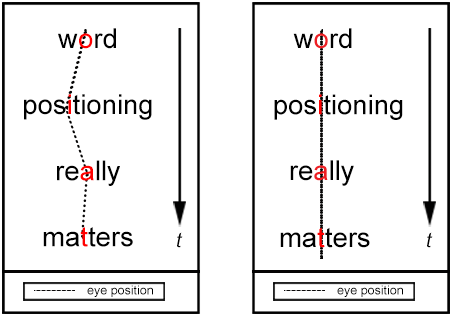
\includegraphics[width=0.3\textwidth]{Pics/opr_spritz}
\caption{Spritz utilizes the optimal recognition position to align words \protect\cite{spritz}.}
\label{fig:spritz_orp}
\end{figure}

\subsection{Critiques of RSVP}
GUSTAV

In order to test how efficient RSVP actually is, a study was conducted by \citeA{schotter_dont_2014}. One thing that is criticized with RSVP techniques is the ability to go back and re-read words for improving one's comprehension. This process is called \textit{regression}, and according to \citeauthor{schotter_dont_2014} about 10\% to 15\% of the time spent reading is by making regressions, i.e. moving eyes back in the text to read material that has previously been processed. The hypothesis is that regression supports reading comprehension, since it allows readers to access more information from the text. This is especially true with texts that are more difficult to read, i.e. that it requires the reader to go back and read words again to make sense of how the sentence is structured. Readers are more likely to make a regression when they sense that their comprehension of the sentence has faltered \cite{schotter_dont_2014}.

By using trailing-mask conditions in their experiment, meaning that whenever a person has read a word, it becomes unreadable by changing it to X's instead, \citeA{schotter_dont_2014} could measure the effects of RSVP (i.e., being shown one word at a time - see Figure \ref{fig:trace_cross}). They found evidence that support the importance of regression. They used a combination of simple sentences and ambiguous garden-path sentences (e.g., "While
the man drank the water that was clear and cold overflowed from the toilet") to investigate when participants tended to regress the most, as well as measure their reading comprehension by answering questions about the sentences. \citeauthor{schotter_dont_2014} found that restricting the opportunity to re-read words with the trailing-mask (replacing the letters with X's) decreased comprehension globally. Unsurprisingly, they also found that participants were significantly more likely to regress in ambiguous sentences, since they had to go back and re-read to understand the sentence properly. Participants made regressions to go back and search for information that would support their overall understanding of the given text. \citeauthor{schotter_dont_2014} also saw evidence that suggests that participants were able to suppress the tendency to re-read, when they knew that regression was not possible due to the trailing-mask system.

\begin{figure}[htbp]
\centering
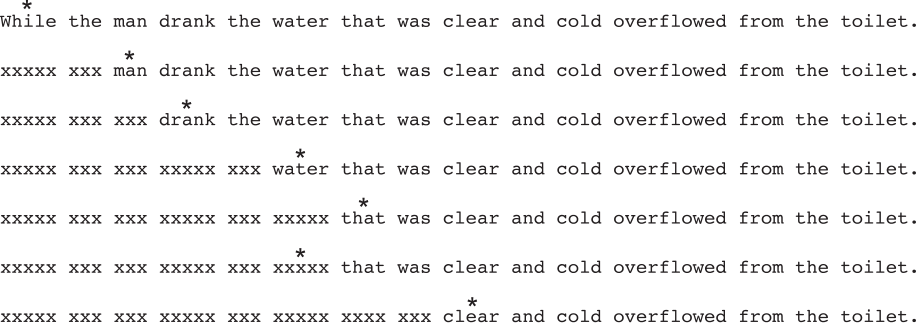
\includegraphics[width=0.4\textwidth]{Pics/trace_crosses}
\caption{Schotter et al. used eye-tracking to mask the words a person had already read, making it impossible to regress. Asterisks represent eye fixations.}
\label{fig:trace_cross}
\end{figure}

\citeauthor{schotter_dont_2014} conclude that reading without the ability to re-read parts of the text, decreases the comprehension accuracy and leads to a poorer understanding of the text.

Loss of spatial awareness and formatting

(INSERT REF) suggests some improvements that should be made to RSVP. One improvement is that it should only present samples of the text, e.g. by selecting only the most informative words of a sentence. This could be determined by only presenting the least frequent content words as well as critical function words. (INSERT REF) also suggests that the duration each word is presented, should be based on an estimate of the processing time for the word. Spritz calculates an estimate by using the shape of the word as well as the length of the word(INSERT SPRITZ REF), however there might be different theories on how to calcuate this \textbf{(Maybe find a better way to write this)}.